% Drawing 154/08-27 -- folder 154, batch 08, archive page 156 (PDF page 157).
% Transcription: en haut à droite, un dessin en couleur : deux configurations réunies par « ou », la droite verte y étant en tirets. À gauche, les tirets passent sous le premier croisement orange (triangle marqué $T$), puis montent pour passer par le second croisement, avec deux flèches vertes (l'une le long des tirets, l'autre transverse, vers le haut) ; à droite, les tirets passent sous le premier croisement (marqué $T$) et par le second, avec une flèche verte vers la droite au-dessus et une flèche transverse vers le bas
% Kind: two configurations joined by « ou »: dashed green line under one orange crossing and through the other, with a pair of green arrows. Method 2 (schematic redraw from the facsimile). Status: ok.
% Notes: Top right of the page; no arrow of the star diagram ends here. Two configurations with « ou » between them. Left: green dashes pass under the first orange crossing (T written in pencil to its left) and rise to the right to go through the second crossing; beyond it two green arrows, one along the dashes and one transverse, pointing up. Right: the dashes pass under the first crossing (T to its left) and through the second; a green arrow to the right above the end of the dashes and a transverse green arrow pointing down below. The dash that goes through each crossing is drawn through the computed crossing (it is hidden under the orange ink there). 8 orange strokes, 4 crossings, 15 dashes, 4 arrows, labels T, T, ou. Read from the 400 dpi colour scan; each pair of orange strokes fitted to the ink and drawn through its computed crossing, the triangles bounded by the computed intersections with the green line; the redraw was overlaid on the scan and agrees to within a stroke's width. The felt strokes are drawn straight (slight curvature of a few strokes not reproduced). Redrawn 2026-11-12 (issue 128): to check again.
% Coordinates: 1 unit = 1 mm = 1/100 of the crop width, same scale on both axes (bbox in page fractions: [0.621, 0.106, 0.934, 0.155]).
% Redrawn by Claude (claude-fable-5-2), issue #128, 2026-11-12; not checked by a human; not compiled (no TeX in the session).
% Rights: reproduces part of the work -- behind RENDER_TRANSCRIPTS, never published by itself.
\documentclass[tikz,border=3pt]{standalone}
\usepackage{amsmath,amssymb}
\usetikzlibrary{patterns,arrows.meta}
\tikzset{Or/.style={orange!90!black}, Lg/.style={green!60!black!70}, Br/.style={brown!80!black}, pencil/.style={black!55}, mpt/.style={circle,draw,inner sep=1.3pt}, pt/.style={circle,fill,inner sep=0.9pt}}
\colorlet{Or}{orange!90!black}\colorlet{Lg}{green!60!black!70}\colorlet{Br}{brown!80!black}
\begin{document}
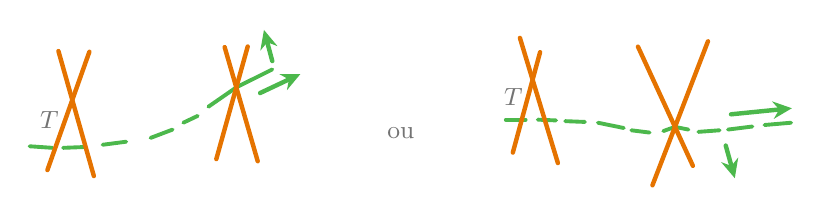
\begin{tikzpicture}[x=1mm,y=1mm,line cap=round,line join=round,font=\scriptsize]
\draw[Lg,line width=1.4pt] (1.45,-16.23) -- (4.35,-16.43);
\draw[Lg,line width=1.4pt] (5.7,-16.43) -- (8.31,-16.33);
\draw[Lg,line width=1.4pt] (10.72,-16.04) -- (13.72,-15.65);
\draw[Lg,line width=1.4pt] (16.81,-15.17) -- (19.61,-14.11);
\draw[Lg,line width=1.4pt] (20.97,-13.24) -- (22.8,-12.37);
\draw[Lg,line width=1.4pt] (24.15,-11.21) -- (27.7,-8.75) -- (32.27,-6.47);
\draw[Or,line width=1.6pt] (5.11,-4.14) -- (6.87,-10.35) -- (9.61,-20.01);
\draw[Or,line width=1.6pt] (9.04,-4.23) -- (6.87,-10.35) -- (3.71,-19.25);
\draw[Or,line width=1.6pt] (26.22,-3.64) -- (27.7,-8.75) -- (30.42,-18.13);
\draw[Or,line width=1.6pt] (29.15,-3.56) -- (27.7,-8.75) -- (25.16,-17.86);
\node[pencil,inner sep=1pt] at (3.96,-12.85) {\small $T$};
\draw[Lg,line width=1.6pt,-{Stealth[length=2.4mm,width=2.2mm]}] (32.27,-5.41) -- (31.21,-1.45);
\draw[Lg,line width=1.6pt,-{Stealth[length=2.4mm,width=2.2mm]}] (30.72,-9.47) -- (35.85,-7.05);
\node[pencil,inner sep=1pt] at (48.6,-14.59) {\small ou};
\draw[Lg,line width=1.4pt] (61.93,-12.85) -- (64.44,-12.85);
\draw[Lg,line width=1.4pt] (65.99,-12.85) -- (68.31,-12.95);
\draw[Lg,line width=1.4pt] (69.47,-13.04) -- (71.98,-13.14);
\draw[Lg,line width=1.4pt] (73.62,-13.24) -- (76.91,-13.91);
\draw[Lg,line width=1.4pt] (77.87,-14.2) -- (80.19,-14.49);
\draw[Lg,line width=1.4pt] (81.93,-14.3) -- (83.41,-13.77) -- (85.12,-14.11);
\draw[Lg,line width=1.4pt] (86.38,-14.4) -- (89.08,-14.2);
\draw[Lg,line width=1.4pt] (90.14,-14.11) -- (93.24,-13.72);
\draw[Lg,line width=1.4pt] (94.78,-13.53) -- (98.16,-13.24);
\draw[Or,line width=1.6pt] (63.72,-2.47) -- (65.33,-7.78) -- (68.54,-18.36);
\draw[Or,line width=1.6pt] (66.28,-4.28) -- (65.33,-7.78) -- (62.82,-17.03);
\draw[Or,line width=1.6pt] (87.6,-2.9) -- (83.41,-13.77) -- (80.55,-21.18);
\draw[Or,line width=1.6pt] (78.71,-3.58) -- (83.41,-13.77) -- (85.69,-18.72);
\node[pencil,inner sep=1pt] at (62.9,-9.95) {\small $T$};
\draw[Lg,line width=1.6pt,-{Stealth[length=2.4mm,width=2.2mm]}] (90.53,-12.17) -- (98.26,-11.4);
\draw[Lg,line width=1.6pt,-{Stealth[length=2.4mm,width=2.2mm]}] (89.86,-16.14) -- (91.01,-20.29);
\end{tikzpicture}
\end{document}
